\section{Funktioner}
A function $f\colon X\to Y$ associates to all $x\in X$ \emph{exactly one} element $ f(x) \in Y$.

\subsection{Function Composition}
If $f\colon X\to Y$ and $g\colon Y\to Z$ then the composition $g\circ f\colon X\to Z$ is defined by $(g\circ f)(x)=g(f(x))$. $f$ is called the \emph{inner function}, $g$ is called the \emph{outer function}
\begin{center}
	\begin{tikzpicture}[scale=0.45]
		\draw \boundellipse{0,0}{0.7}{1.4};
		\draw\boundellipse{5,0}{0.7}{1.4};
		\draw\boundellipse{10,0}{0.7}{1.4};
		\node at (0.45,1.7) [label=left:$X$]{};
		\node at (5.45,1.7) [label=left:$Y$]{}; 
		\node at (10.45,1.7) [label=left:$Z$]{}; 
		\node[circle, fill,inner sep=1pt] (x) at (0.05,0) [label=below:$x$]{};
		\node[circle, fill,inner sep=1pt] (fx) at (5.05,0) [label=below:$f(x)$]{};
		\node[circle, fill,inner sep=1pt] (gfx) at (10.05,0) [label=below:$g(f(x))$]{};
		\draw[thick,->,blue] (x) to [bend right] node[pos=0.5, label=below:$f$] {} (fx) ;
		\draw[thick,->,red] (fx) to [bend right] node[pos=0.5, label=below:$g$] {} (gfx) ;
		\draw[thick,->,purple] (x) to [bend left] node[pos=0.25, label=above:$g\circ f$] {} (gfx) ;
\end{tikzpicture}%
\end{center}
\subsection{Inverse Functions}
Two functions $f\colon X\to Y$ and $g\colon Y\to X$ are \emph{inverse functions} if
\begin{align*}
f(g(y))=y,\quad \textup{and}\quad g(f(x))=x 
\end{align*}
for all $x$ in $X$ and $y$ in $Y$.

\begin{center}
\begin{tikzpicture}[scale=0.7]
\draw \boundellipse{0,0}{0.7}{1.4};
\draw \boundellipse{5,0}{0.7}{1.4};
\node at (0.45,1.7) [label=left:$X$]{};
\node at (5.45,1.7) [label=left:$Y$]{}; 
\node[circle,fill,inner sep=1pt] (x) at (0,1) [label=below:$x$] {};
\node[circle,fill,inner sep=1pt] (gy) at (0,-1) [label=above:$g(y)$] {};
\node[circle,fill,inner sep=1pt] (fx) at (5,1) [label=below:$f(x)$] {};
\node[circle,fill,inner sep=1pt] (y) at (5,-1) [label=above:$y$] {};
\draw[thick,->,blue] (x) to[bend left]node[pos =0.5, label=above:$f$] {} (fx);
\draw[thick,->,red] (fx) to[bend left] node[pos =0.5, label=above:$g$] {} (x);
\draw[thick,->,red] (y) to[bend left]node[pos =0.5, label=below: $g$] {} (gy);
\draw[thick,->,blue] (gy) to[bend left]node[pos =0.5, label=below: $f$] {} (y);
\end{tikzpicture}%
\end{center}

\subsection{Polynomials}
A first order polynomial is on the form:
\begin{align*}
f(x)=ax+b.
\end{align*}
A second order polynomial is on the form:
\begin{align*}
f(x)=ax^2+bx+c.
\end{align*}
\subsection{Logarithms and Exponential Functions}
The \emph{logarithm with base $a$}, $\log_a\colon ]0,\infty[\to \R$ is inverse to the exponential function $f_a(x)=a^x$ ($a>0$, $a\neq 1$). We have that
\begin{align*}
\log_a(a^x)=x\quad \textup{and} \quad a^{\log_a(y)}=y
\end{align*}
and that
\begin{align*}
\ln x=\log_e x,&& \log x=\log_{10} x
\end{align*}
\subsection{Rules}
We have that
\begin{align*}
\log_a(xy)&=\log_a(x)+\log_a(y),\\\log_a\Big(\frac{x}{y}\Big)&=\log_a(x)-\log_a(y),\\ \log_a(x^r)&=r\log_a(x).
\end{align*}
\section{Trigonometric Functions}
The trigonometric functions are defined by using the unit circle:
\begin{center}
	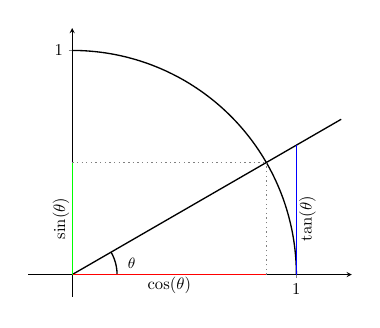
\begin{tikzpicture}[scale=0.6]
	\begin{axis}[xmin=-0.05,xmax=1.1,ymin=-0.1,ymax=1.1,axis x line=center,
	axis y line=center, axis equal, xtick={0,1},ytick={0,1}]
	%PERMANENT STUFF
	\addplot[domain=0:pi/2,thick, samples=100] ({cos(deg(x))},{sin(deg(x))});
	\addplot[domain=0:sqrt(3)/2,thick] {1/sqrt(3)*x};
	\addplot[domain=0:pi/6,thick,samples=100] ({0.2*cos(deg(x))},{0.2*sin(deg(x))}) node[label=right:{\small$\theta$},pos=0.5] {};
	%cos
	\addplot[dotted,gray,thick] coordinates {(sqrt(3)/2,0) (sqrt(3)/2, 1/2)};
	\node at (axis cs: {sqrt(3)/4},-0.05) {$\cos(\theta)$};
	\addplot[thick,red,domain=0:sqrt(3)/2] {0};
	%sin
	\node at (axis cs: -0.05,1/4) {\rotatebox{90}{$\sin(\theta)$}};
	\addplot[dotted, gray,thick,domain=0:sqrt(3)/2] {1/2};	
	\addplot[thick,green]  coordinates { (0,0) (0,1/2)};
	%tan
	\addplot[thick,domain=sqrt(3)/2:1.2] {1/sqrt(3)*x};
	\node at (axis cs: 1.05,1/4) {\rotatebox{90}{$\tan(\theta)$}};
	\addplot[blue,thick] coordinates {(1,0) (1, 1/sqrt(3)};
	\end{axis}
	\end{tikzpicture}%
\end{center}
We have that
\begin{center}
\begin{tabular}{@{} lccccc @{}}
	\toprule 
	$\theta$			& 0			&$ \frac{\pi}{6} $  		&$ \frac{\pi}{4} $ 		&$ \frac{\pi}{3}$ 			&$ \frac{\pi}{2} $		\\ \midrule
	$\sin \theta$		&0			&$ \frac{1}{2} $			&$ \frac{\sqrt{2}}{2} $	& $ \frac{\sqrt{3}}{2} $ 	& 1						\\ \midrule
	$\cos \theta$		&1			&$\frac{\sqrt{3}}{2}$		&$\frac{\sqrt{2}}{2}$	& $\frac{1}{2}$				&0	\\ \midrule
	$\tan \theta$		&0			&$\frac{1}{\sqrt{3}}$		&$1$					& $ \sqrt{3} $				&-		\\ \midrule
\end{tabular}
\end{center}
and that $ \tan(\theta)=\frac{\sin(\theta)}{\cos(\theta)}$.





%\begin{tabular}{@{} lccc @{}}
%	\toprule 
%	$\theta$			& $\sin \theta$			& $\cos \theta$ 		& $\tan \theta$ 		\\ \midrule
%	0					&0						&1						&0						\\ \midrule
%	$ \frac{\pi}{6} $	&$\frac{1}{2}$			&$\frac{\sqrt{3}}{2}$	&$\frac{1}{\sqrt{3}}$	\\ \midrule
%	$ \frac{\pi}{4} $	&$\frac{\sqrt{2}}{2}$	&$\frac{\sqrt{2}}{2}$	&$1$					\\ \midrule
%	$ \frac{\pi}{3} $	&$\frac{\sqrt{3}}{2}$	&$\frac{1}{2}$			&$\sqrt{3}$				\\ \midrule
%	$ \frac{\pi}{2} $	&1						&0						&						\\ \bottomrule  
%\end{tabular}

















